\section{Capítulo 6: Confiabilidad y tolerancia a fallos}

\textbf{Confiabilidad:} La confianza que se puede tener en un sistema, aun en presencia de errores, fallos y condiciones inesperadas.

Atributos claves

\begin{enumerate}
    \item \textcolor{red}{\textbf{Fiabilidad:}} Continuidad correcta del servicio sin fallas o interrupciones.
    \item \textcolor{red}{\textbf{Disponibilidad:}} La disposición de un servicio a ser usado en cualquier tiempo \textbf{T} .
    \item \textcolor{red}{\textbf{Mantenibilidad:}} Facilidad de mantener, actualizar y reparar un sistema que puede fallar.
    \item \textcolor{red}{\textbf{Protección:}} Ausencia de consecuencias catastróficas sobre el medio ambiente.
    \item \textcolor{red}{\textbf{Seguridad}} Prevenir el acceso o manipulación no autorizaco (alineado con la \textcolor{red}{\textbf{CIA: Confidencialidad, Integridad y Disponibilidad}}).
\end{enumerate}

Los atributos antes mencionados son cuantificables y medibles para el analisis de la \textbf{tolerancia a fallos}.

\subsubsection{Modelo Causal de averias}
Para este contexto definiremos al sistema como un conjunto de componentes tanto de hardware como de software, preparados para colaborar coordinadamente para ofrecer un servicio, según pautas establecidas para un correcto funcionamiento.

\begin{figure}[H]
    \centering
    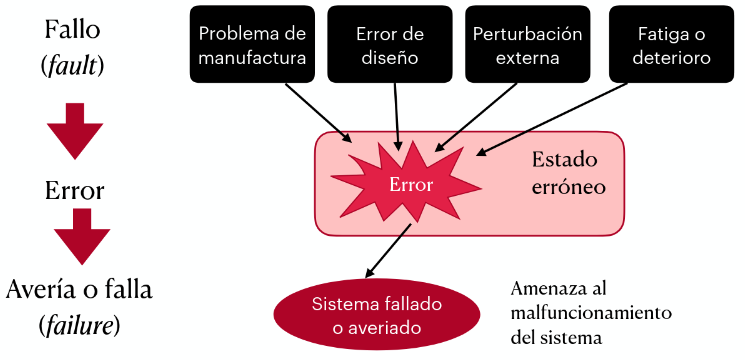
\includegraphics[width=0.48\linewidth]{img/Modelo_Causal_de_averias.png}
    \caption{Modelo Causal de averias}\label{fig:1761579857293}
\end{figure}

Pero, que causa un mal funcionamiento de un sistema. Partiremos definiendo 3 diferencias claves para el analisis.

\begin{itemize}
    \item \textcolor{red}{\textbf{Fallo(\textit{fault}):}} Defecto o funcionamiento anormal de un componente, el cual tiene el potencial de causar un \textcolor{red}{\textbf{error}}, en caso de no ser tratado \textcolor{red}{\textbf{puede llevar a una averia}}. Se clasifican segun persistencia (\textcolor{red}{\textbf{transistente, intermitente o permanente}}) y según causa \textcolor{red}{\textbf{error de manofactura, diseño u operacional}} 
    \item \textcolor{red}{\textbf{Error:}} Discrepancia entre el comportamiento esperado y el exhibido
    \item \textcolor{red}{\textbf{Averia(\textit{failture}):}} Ocurre un malfuncionamiento que conduce a que ya no se pueda proveer el servicio especificado. Son causadas por errores que se propagar a lo largo del sistema, llegando a ser observables por el usuario.
    \subitem \textbf{Un error o fallo no necesariamente conduce a una averia, si este es tratado y manejado adecuadamente}
\end{itemize}

Las \textbf{\textit{fallas}} o \textbf{\textit{averias}} se clasifican según su comportamiento en el sistema

\begin{itemize}
    \item Fallas de \textcolor{red}{\textbf{caida (\textit{crash}):}} Componente se detiene y no se recupera por si mismo
    \subitem \textcolor{red}{\textbf{Proceso:}} Proceso fallado se detiene, puede perder su estado. Es la mas benigna es detenerse manteniendo su estado, para posteriormente recuperarlo. Para la detenccion fiable por parte de otros procesos se requieren \textcolor{red}{\textit{timers}}
    \subitem \textcolor{red}{\textbf{Comunicación:}} Falla del sistema de comunicación con pérdida continua de mensajes (e.g falla permanenete o partición de red)

    \item Fallas de \textcolor{red}{\textbf{omisión:}} El sistema no responde transitoriamente
    \subitem \textcolor{red}{\textbf{Proceso:}} Proceso no responde, sin perder estado \textcolor{red}{(e.g., se pierde una solicitud de servicio)}.
    \subitem \textcolor{red}{\textbf{Comunicación:}} Se pierden algunos mensajes. Falla mas benigna es que mensajes no se corrompen (integridad) y no se puede falsear su
    remitente (autenticidad). Recuperación es por retransmisión de mensajes perdidos.

    \item Fallas \textcolor{red}{\textbf{temporales (\textit{timing}):}} El sistema no responde dentro de los limites de tiempo.
    \subitem Pueden corresponder a un mal desempeño por sobrecarga. 
    \subitem Pueden ocurrir por fallas de relojes.

    \item Fallas \textcolor{red}{\textbf{arbitrarias (\textit{bizantinas}):}} El sistema se comporta inconsistente o maliciosamente.
    \subitem Los procesos fallas siguen funcionando pero no garantizan la integridad de los mensajes \textcolor{red}{\textbf{(peor caso)}}
    \subitem A veces se produce por corrupción interna del sistema, causan respuestas erroneas pero no maliciosas
    \subitem Son fallas dificiles de detectar y tolerar
\end{itemize}

Una vez definidas el tipo de fallas, estableceremos los modelos para los tipos de fallas, en base a una jerarquia.
\begin{figure}[H]
    \centering
    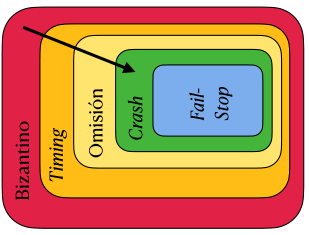
\includegraphics[width=0.3\linewidth]{img/modelo_de_fallas.png}
    \caption{Modelo de fallas}\label{fig:1761584179354}
\end{figure}

\begin{itemize}
    \item \textcolor{red}{\textbf{Fail-stop:}} Un proceso fallado se detiene, conservando su estado, y todos los demas saben inmediatamente que ha fallado. Los procesos se comportan correctamente o se detienen.
    \item \textcolor{red}{\textbf{Crash:}} Modelo realista de incertidumbre para sistemas asincronicos. Un proceso fallad se detiene, conserva su estado, pero los demans no lo saben ni estan seguros si se cayo o esta lento o tiene problemas de comunicación. Puede recuperarse y reintegrarse al sistema
    \item \textcolor{red}{\textbf{Omisión:}} Solo un proceso puede omitir enviar o recibir mensajes. Se puede abordar con el uso de timers, reintento y asentimientos.
    \item \textcolor{red}{\textbf{Temporal (\textit{timing}):}} El sistema puede violar restricciones temporales, tal como respuestas fuera de tiempo. Dificil de discriminar entre fallas de crash y omisión
    \item \textcolor{red}{\textbf{Bizantino:}} Un proceso puede enviar mensajes contradictorios, mentir sobre su estado interno o colaborar maliciosamente con otros. Corresponde a un modelo más general
\end{itemize}

Para manejar lo anterior, se propone los siguientes enfoques para mejorar la confiabilidad del sistema.

\begin{itemize}
    \item \textcolor{red}{\textbf{Prevención de fallos:}} Prevenir que ocurran o se introduzcan fallos en el sistema
    \item \textcolor{red}{\textbf{Remoción de fallos}} durante el desarrollo o durante el uso \textbf{(mantencion y reparacion)}
    \item \textcolor{red}{\textbf{Pronóstico de fallos:}} Predecir fallos probables, para que puedan ser anticipadamente eliminadas o contener sus efectos \textbf{(e.g. alertas y detección de degradación/anomalías)}
    \item \textcolor{red}{\textbf{Pronóstico de fallos:}} Capacidad de un sistema para seguir funcionando normalmente, aun cuando seproduzcan uno o más fallos de sus componentes.
    \subitem Se debe disponer de algún tipo de redundancia para enmascarar fallos.
    \subitem Capacidad de reparar un fallo sin interrumpir el servicio, para asegurar continuidad operacional del servicio.
\end{itemize}
